\chapter{Evaluation}
\label{chapter_evaluation}

\section{Running time}

For the running time evaluation we used a computer with 16 GB RAM and The Intel(R) Core(TM) i7-3770 CPU @ 3.40GHz. The source code was compiled with \lstinline|gcc| 4.8.2 and the \lstinline|-O3| flag to enable compiler optimizations.

First we give an overview of running time on different graphs with variable choice of parameters $k$ (as in $k$-bond) and $m$ (maximum size of a bond). These running times were measured using the GNU \lstinline|time| utility. Time spent interacting with the operating system was not included in the measurement.

Then we show how much time is spent generating the $k$-bonds from edge $e \in F$, where $F$ is the spanning forest chosen in the first steps of the algorithm. Here $\mtime(e)$ is the number of milliseconds the program runs in the branch of computation starting with $X = \{e\}$ and $\mbonds(e)$ is the number of bonds it generated, $Q_p$ is $p$-th quantile of the time attribute of the data set. Based on the following $\chi$ function, we define $\mathcal{P}(x,y) = \{ e \in F : \chi(x,y,e) = 1 \}$ and $\#Q_x, Q_y = \lvert \mathcal{P}(x,y) \rvert$.

\[
	\chi(x, y, e) \stackrel{\text{def}}{=}
	\begin{cases}
		\hfill 1  \hfill & \text{\textbf{if} $Q_x < \mtime(e) \leq Q_y$ \break \textbf{or} $x=0 \wedge \mtime(e) = Q_x$,} \\
		\hfill 0  \hfill & \text{otherwise} \\
	\end{cases}
\]

\[
	\Sigma Q_x, Q_y \stackrel{\text{def}}{=} \sum_{e \in \mathcal{P}(x,y)} \mbonds(e)
\]

To measure elapsed $\mtime$ we are using \lstinline|process_user_cpu_clock| from the \lstinline|boost::chrono| \thinspace C++ library. This clock reports CPU time spent by the current process in the user space (i.e.\ the time interacting with the operating system was not included).


\clearpage

%%% Runtime Zlin

\subsection*{Zlín Region (723 vertices, 974 edges)}

In Figure \ref{fig:zlin_rtm} we can see how the time taken depends on the number of bonds produced when generating a family of bonds (all bonds in the family having a common first edge). Table \ref{table:zlin-rtm-stat} shows that the quarter of the longest taking computations generate the majority of bonds.


\begin{table}[H]
	\caption{Running time in seconds for different choices of $k$ (rows) and $m$ (columns)}
	\centering
	\begin{tabular}{c|rrrrrrrr}

\toprule

	&         2 &         3 &         4 &         5 &         6 &         7 &		8 	\\ \midrule
 2	&      0.03 &      0.10 &      0.40 &      1.69 &      8.47 &     42.60 &	210.34	\\
\evenrowcolor
 3	&      0.57 &      2.77 &     12.50 &     53.38 &    223.15 &    986.02 &	4603.89	\\
 4	&           &     29.49 &    197.92 &   1018.22 &   4771.04 &  21269.76 &	-		\\
\evenrowcolor
 5	&           &           &   1155.52 &   9884.54 &  56847.00 &	-	   & 	-		\\

	\end{tabular}
\end{table}

\vspace{-0.5cm}
\begin{figure}[H]
	\caption{Each point represents the process of generating bonds starting with an edge of the $k$-way basis, here $k = 4$ and $m = 4$}
	\label{fig:zlin_rtm}

	\centering
	\begin{gnuplot}[terminal=epslatex, terminaloptions=color]
		unset key

		set style line 1 lc rgb 'black' pt 2   # square
		set style line 12 lc rgb'#808080' lt 0 lw 1
		set grid back ls 12

		set xtics nomirror rotate by -45
		set format x '%.0s %c'

		set xlabel "Number of generated $k$-bonds"
		set ylabel "Time to taken (ms)"
		plot "data/rtm/rtm-zlin-4-4-d1.dat" using 3:2 with points ls 1
	\end{gnuplot}
\end{figure}

\vspace{-1cm}

\begin{table}[H]
	\caption{Statistics of the data set used in Figure \ref{fig:zlin_rtm}. Computations with $\mtime(e) = \mbonds(e) = 0$ excluded}
	\label{table:zlin-rtm-stat}
	\centering
	\begin{tabular}{rr||rr|r|r}

\toprule
$p_1$	&	$p_2$		& $Q_{p_1}$	& $Q_{p_2}$	& $ \#Q_{p_1},Q_{p_2} $ & $ \Sigma Q_{p_1},Q_{p_2} $ \\ \midrule

0	&	0.25	& 0	&	110	& 72	& 44753 \\
\evenrowcolor
0.25	&	0.5	& 110	&	340	& 70	& 262593 \\
0.5	&	0.75	& 340	&	1175	& 70	& 678110 \\
\evenrowcolor
0.75	&	1	& 1175	&	9730	& 71	& 2858919 \\

	\end{tabular}
\end{table}


%%% Runtime Olomouc

\subsection*{Olomouc Region (1454 vertices, 2066 edges)}

In the Olomouc Region a bigger part of the resulting bonds is generated by the quarter of the edges with the lowest $\mtime(e)$ than in Zlín Region. This can be seen in Figure \ref{fig:olomouc_rtm} and Table \ref{table:olomouc-rtm-stat}.

\begin{figure}[H]
	\caption{Each point represents the process of generating bonds starting with an edge of the $k$-way basis, here $k = 3$ and $m = 7$}
	\label{fig:olomouc_rtm}

	\centering
	\begin{gnuplot}[terminal=epslatex, terminaloptions=color]
		unset key

		set style line 1 lc rgb 'black' pt 2   # square
		set style line 12 lc rgb'#808080' lt 0 lw 1
		set grid back ls 12

		set xtics nomirror rotate by -45
		set format x '%.0s %c'

		set xlabel "Number of generated $k$-bonds"
		set ylabel "Time to taken (ms)"
		plot "data/rtm/rtm-olomouc-7-3-d1.dat" using 3:2 with points ls 1
	\end{gnuplot}
\end{figure}

For clarity Figure \ref{fig:olomouc_rtm_under30k_ms} displays the same data as Figure \ref{fig:olomouc_rtm} but without the very few records with long time and a great number of bonds produced. We see that the ratio of time taken and number of bonds generated is higher than desirable in some cases.

\begin{figure}[H]
	\caption{Data from Figure \ref{fig:olomouc_rtm} but only records with $\mtime < 30000$ are displayed}
	\label{fig:olomouc_rtm_under30k_ms}

	\centering
	\begin{gnuplot}[terminal=epslatex, terminaloptions=color]
		unset key

		set style line 1 lc rgb 'black' pt 2   # square
		set style line 12 lc rgb'#808080' lt 0 lw 1
		set grid back ls 12

		set xtics nomirror rotate by -45
		set format x '%.0s %c'

		set xlabel "Number of generated $k$-bonds"
		set ylabel "Time to taken (ms)"
		plot "data/rtm/rtm-olomouc-7-3-d1-under30k-ms.dat" using 3:2 with points ls 1
	\end{gnuplot}
\end{figure}

\vspace{-1cm}

\begin{table}[H]
	\caption{Running time in seconds for different choices of $k$ (rows) and $m$ (columns)}
	\centering
	\begin{tabular}{c|rrrrrrrr}

\toprule

        &         1 &         2 &         3 &         4 &         5 &         6 &      7 &      8 \\
\midrule
     2  &      0.02 &      0.07 &      0.30 &      1.28 &      5.15 &     16.16 &     69 &    305 \\
\evenrowcolor
     3  &           &      3.00 &     10.38 &     60.88 &    235.40 &    921.45 &   3482 &  13342 \\
     4  &           &           &    158.29 &    781.43 &   6008.40 &        -  &      - &      - \\
\evenrowcolor
     5  &           &           &           &   6205.22 &  43242.26 &        -  &      - &      - \\



	\end{tabular}
\end{table}


\begin{table}[H]
	\caption{Statistics of the data set used in Figure \ref{fig:olomouc_rtm}. Table excludes computations with $\mtime(e) = \mbonds(e) = 0$}
	\label{table:olomouc-rtm-stat}
	\centering
	\begin{tabular}{rr||rr|r|r}

\toprule
$p_1$	&	$p_2$		& $Q_{p_1}$	& $Q_{p_2}$	& $ \#Q_{p_1},Q_{p_2} $ & $ \Sigma Q_{p_1},Q_{p_2} $ \\ \midrule

0	&	0.25	& 0	&	515	& 358	& 639245 \\
\evenrowcolor
0.25	&	0.5	& 515	&	1290	& 361	& 2257757 \\
0.5	&	0.75	& 1290	&	2980	& 354	& 4128353 \\
\evenrowcolor
0.75	&	1	& 2980	&	104450	& 358	& 12456337 \\
	\end{tabular}
\end{table}



%%% Runtime Stredocesky

\subsection*{Central Bohemian Region (4114 vertices, 5964 edges)}

Measurements with the road network of the Central Bohemian (Středočeský) Region have similar results as those with the Olomouc Region road network. In figures \ref{fig:stredocesky_rtm} and \ref{fig:stredocesky_rtm_4_3} each point represents the process of generating bonds starting with an edge of the $k$-way basis. Figure \ref{fig:stredocesky_rtm} shows an increased number of comparatively slower computations, however this is not significant for greater $m$ as can be seen in \ref{fig:stredocesky_rtm_4_3}.


\begin{table}[H]
	\caption{Statistics of the data set used in Figure \ref{fig:stredocesky_rtm}. Computations with $\mtime(e) = \mbonds(e) = 0$ excluded}
	\label{table:stredocesky-rtm-stat}
	\centering
	\begin{tabular}{rr||rr|r|r}

\toprule
$p_1$	&	$p_2$		& $Q_{p_1}$	& $Q_{p_2}$	& $ \#Q_{p_1},Q_{p_2} $ & $ \Sigma Q_{p_1},Q_{p_2} $ \\ \midrule

0	&	0.25	& 0	&	60	& 240	& 20252 \\
\evenrowcolor
0.25	&	0.5	& 60	&	120	& 216	& 54499 \\
0.5	&	0.75	& 120	&	230	& 209	& 85212 \\
\evenrowcolor
0.75	&	1	& 230	&	560	& 218	& 152298 \\


	\end{tabular}
\end{table}


\begin{table}[H]
	\caption{Running time in seconds for different choices of $k$ (rows) and $m$ (columns)}
	\label{fig:stredocesky_kmvar}
	\centering
	\begin{tabular}{c|rrrrrrrr}

\toprule
        &         1 &         2 &         3 &         4 &         5 &      6 &         7 &         8 \\
\midrule
     2  &      0.24 &      0.72 &      3.85 &     12.71 &     37.85 &    140 &    599 &   2687 \\
\evenrowcolor
     3  &           &     47.32 &    175.76 &   1156.88 &   4480.29 &  18366 &           &           \\

	\end{tabular}
\end{table}


\begin{figure}[H]
	\caption{$k = 3$ and $m = 3$}
	\label{fig:stredocesky_rtm}

	\centering
	\begin{gnuplot}[terminal=epslatex, terminaloptions=color]
		unset key

		set style line 1 lc rgb 'black' pt 2   # square
		set style line 12 lc rgb'#808080' lt 0 lw 1
		set grid back ls 12

		set xtics nomirror rotate by -45
		set format x '%.0s %c'

		set xlabel "Number of generated $k$-bonds"
		set ylabel "Time taken (ms)"
		plot "data/rtm/rtm-stredocesky-3-3-d1.dat" using 3:2 with points ls 1
	\end{gnuplot}
\end{figure}

\vspace{-1cm}

\begin{figure}[H]
	\caption{$k = 3$, $m = 4$}
	\label{fig:stredocesky_rtm_4_3}

	\centering
	\begin{gnuplot}[terminal=epslatex, terminaloptions=color]
		unset key

		set style line 1 lc rgb 'black' pt 2   # square
		set style line 12 lc rgb'#808080' lt 0 lw 1
		set grid back ls 12

		set xtics nomirror rotate by -45
		set format x '%.0s %c'

		set xlabel "Number of generated $k$-bonds"
		set ylabel "Time taken (ms)"
		plot "data/rtm/rtm-stredocesky-4-3-d1.dat" using 3:2 with points ls 1
	\end{gnuplot}
\vspace{-1cm}
\end{figure}

\subsection*{Running time according to graph density}

We show how the number of edges of the given graph affects the time taken generating the bonds. However the figures also show that the number of bonds of given size quickly decreases in denser graphs. The running time decreases too becaus finding the unique shortest path is quick in a dense graph.


\begin{figure}[H]
	\caption{Graphs on 25 vertices, $k = 4$ and $m = 15$}
	\label{fig:density_times}

	\centering
	\begin{gnuplot}[terminal=epslatex, terminaloptions=color]
		unset key

		set style line 1 lc rgb 'black' pt 2   # square
		set style line 12 lc rgb'#808080' lt 0 lw 1
		set grid back ls 12

		set xtics nomirror rotate by -45
		set format x '%.0s %c'

		set ylabel "Time taken (ms)"
		set xlabel "The number of edges in the graph"
		plot "data/density/density-15-4.dat" using 1:2 with points ls 1
	\end{gnuplot}
\end{figure}


\begin{figure}[H]
	\caption{Number of generated bonds (the same data set as in \ref{fig:density_times})}
	\label{fig:density_bonds}

	\centering
	\begin{gnuplot}[terminal=epslatex, terminaloptions=color]
		unset key

		set style line 1 lc rgb 'black' pt 2   # square
		set style line 12 lc rgb'#808080' lt 0 lw 1
		set grid back ls 12

		set xtics nomirror rotate by -45
		set format x '%.0s %c'

		set ylabel "Number of generated bonds"
		set xlabel "The number of edges in the graph"
		plot "data/density/density-15-4.dat" using 1:3 with points ls 1
	\end{gnuplot}
\vspace{-1cm}
\end{figure}

%%%%%%%%%% EFFECTS OF CANONICAL

\section{Acceleration with canonical generation}

We compare the number of generated bonds (including more permutations of the same bond, see section below) with and without canonical generation. Canonical generation was disabled by removing all conditions (introduced in Chapter \ref{ch:canonical}) which resulted in pruning of the search space.

\subsection*{Zlín Region}

\begin{table}[H]
	\caption{How many times is the canonical generation faster for given $k$ (rows) and $m$ (columns)}
	\centering
	\begin{tabular}{c|rrrrrrrr}

\toprule

         &         2 &         3 &         4 &         5 &         6 &         7 \\
\midrule
      2  &        1  &         2 &      2.45 &      3.60 &       4.3 &      1.34 \\
\evenrowcolor
      3  &      3.28 &      3.51 &      6.05 &      8.83 &     12.11 &     14.90 \\
      4  &           &       8.4 &     11.32 &     15.73 &         - &         - \\

	\end{tabular}
\end{table}

\begin{table}[H]
	\caption{How much less ordered bonds does the canonical generation produce for given $k$ (rows) and $m$ (columns)}
	\centering
	\begin{tabular}{c|rrrrrrrr}

\toprule

        &         2 &         3 &         4 &         5 &         6 &         7 \\ \midrule
     2  &      1.43 &      1.97 &      2.67 &      3.52 &      4.42 &      1.15 \\
\evenrowcolor
     3  &      2.00 &      3.08 &      4.27 &      5.99 &      7.94 &     10.09 \\
     4  &           &      6.00 &      9.50 &     13.38 &         - &         - \\


	\end{tabular}
\end{table}


\subsection*{Olomouc Region}


\begin{table}[H]
	\caption{How many times is the canonical generation faster for given $k$ (rows) and $m$ (columns)}
	\centering
	\begin{tabular}{c|rrrrrrrr}

\toprule

   &         2 &         3 &         4 &         5 &         6 &     7 &     8 \\ \midrule
2  &      1.14 &      1.93 &      1.91 &      2.18 &      4.30 &  5.06 &  5.57 \\
\evenrowcolor
3  &      1.97 &      3.47 &      4.49 &      6.69 &      8.31 &     - &     - \\
4  &           &      5.96 &     10.16 &     15.53 &         - &     - &     - \\

	\end{tabular}
\end{table}

\begin{table}[H]
	\caption{How much less ordered bonds does the canonical generation produce for given $k$ (rows) and $m$ (columns)}
	\centering
	\begin{tabular}{c|rrrrrrrr}

\toprule

   &      2 &         3 &         4 &         5 &         6 &         7 &         8 \\ \midrule
2  &   1.32 &      1.93 &      2.53 &      3.26 &      4.04 &      4.78 &      5.51 \\
\evenrowcolor
3  &   2.00 &      2.84 &      4.03 &      5.50 &      7.41 &         - &         - \\
4  &        &      6.00 &      8.79 &     12.37 &        -  &         - &         - \\



	\end{tabular}
\end{table}

%%% Failed to canonize:


\section*{Generated non-canonical permutations}

If we consider canonicity with respect to each bond, not bond and its certain partition as in the definition of $\mcan()$, our algorithm still generates more permutations of the same bond. Due to its complexity and (as demonstrated below) little impact on the result, the algorithm does not perform an explicit isomorphism test for each generated bond. We show an example and document how much is the result non-canonical.

\begin{figure}[H]
	\caption{Let $k = 3$, $m = 3$. In stage 1 the algorithm generates bonds 0,1 and 0,2. In stage 2 bond 0,1 is extended to 0,1,2 and bond 0,2 is extended to 0,2,1. }
\begin{center}
	% 
% dot2tex --autosize tmp/graph9.tmp --prog neato --figonly
%

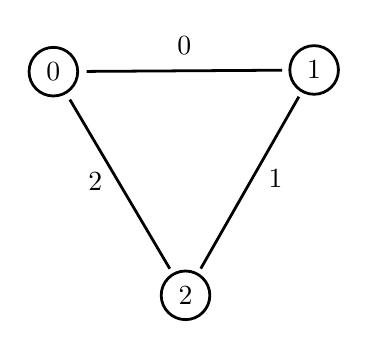
\begin{tikzpicture}[>=latex,line join=bevel,real/.append style={circle, draw=black} ]
  \pgfsetlinewidth{1bp}
%%
\pgfsetcolor{black}
  % Edge: 0 -- 1
  \draw [] (-35.2bp,26.724bp) .. controls (-15.446bp,26.841bp) and (15.392bp,27.043bp)  .. (35.2bp,27.159bp);
  \definecolor{strokecol}{rgb}{0.0,0.0,0.0};
  \pgfsetstrokecolor{strokecol}
  \draw (0bp,35.941bp) node {0};
  % Edge: 2 -- 0
  \draw [] (-5.2199bp,-44.329bp) .. controls (-14.277bp,-29bp) and (-31.973bp,0.95243bp)  .. (-41.211bp,16.588bp);
  \draw (-32.1bp,-12.8705bp) node {2};
  % Edge: 1 -- 2
  \draw [] (41.229bp,17.623bp) .. controls (32.319bp,2.0092bp) and (14.815bp,-28.662bp)  .. (5.9095bp,-44.269bp);
  \draw (32.8bp,-12bp) node {1};
  % Node: 1
\begin{scope}
  \definecolor{strokecol}{rgb}{0.0,0.0,0.0};
  \pgfsetstrokecolor{strokecol}
  \draw (46.722bp,27.249bp) node [real] {1};
\end{scope}
  % Node: 0
\begin{scope}
  \definecolor{strokecol}{rgb}{0.0,0.0,0.0};
  \pgfsetstrokecolor{strokecol}
  \draw (-47.146bp,26.633bp) node [real] {0};
\end{scope}
  % Node: 2
\begin{scope}
  \definecolor{strokecol}{rgb}{0.0,0.0,0.0};
  \pgfsetstrokecolor{strokecol}
  \draw (0.42374bp,-53.881bp) node [real] {2};
\end{scope}
%
\end{tikzpicture}


\end{center}
\end{figure}

\vspace{-0.5cm}

We measure how often multiple generation happens when processing real-world road networks. The tables show increase in the number of generated bonds (compared to the number of unique \linebreak bonds) in percent. The bound on the number of edges in the cuts changes with columns, the multiplicity of the cut changes with rows.

\begin{table}[H]
	\caption{Zlín Region -- $4$-bonds with up to $7$ edges, increase in \%}
	\centering
	\begin{tabular}{c|rrrrrrrr}

\toprule

          &        3 &         4 &         5 &         6 &         7 \\ \midrule
       3  &    0,972 &     0,814 &     1,618 &     2,664 &     3,715 \\
\evenrowcolor
       4  &          &     2,177 &     1,950 &     3,462 & -   \\

	\end{tabular}
\end{table}


\begin{table}[H]
	\caption{Olomouc Region -- $4$-bonds with up to $7$ edges, incr. in \%}
	\centering
	\begin{tabular}{c|rrrrrrrr}

\toprule

            &         3 &         4 &         5 &         6 &         7 \\ \midrule
         3  &     0,156 &     0,253 &     0,649 &     1,049 &     1,568 \\
\evenrowcolor
         4  &           &     0,352 &     0,541 &         -  &       -  \\

	\end{tabular}
\end{table}

\clearpage

\section{Properties of shortest paths}

\subsection*{Number of shortest paths with equal $\mlen_\lambda$}

Two shortest $V(T_r){-}V_b$ paths $P_1, P_2$ can satisfy $\mlen_\lambda(P_1) = \mlen_\lambda(P_2)$. This is undesirable since our aim is to randomize the selection and the lexicographical comparison of the vectors of the edge indicies is just a saftey measure. However our measurements were unable to record a case of said equality. The following settings were used:

\begin{itemize}
	\item Zlín Region, $(k, m) \in \{1,\ldots,4\} \times \{1,\ldots,5\}$ and $k=2, m \leq 8$
	\item Olomouc Region, $(k, m) \in \{1,\ldots,4\} \times \{1,\ldots,4\}$
	\item Central Bohemian Region, $(k, m) \in \{1,\ldots,3\} \times \{1,\ldots,4\}$
\end{itemize}

\subsection*{Length of paths in various stages}

Following measurements show the average length of found shortest $V(T_r){-}V_b$ path according to stage number (in the rows) and number of \lstinline|GenStage| calls on the call stack (in the columns). Paths of length $0$ (that is when no path is found) are not included in these statistics.

\begin{table}[H]
	\caption{Zlín Region -- $4$-bonds with up to 6 edges}
	\centering
	\begin{tabular}{c|rrrr}
		\toprule
		        & 1    & 2    & 3  	 & 4	  \\ \hline
		1       & 5.41 & 5.71 & 5.87 & 6.00  \\
		\evenrowcolor
		2       & 4.82 & 5.39 & 5.46 & 5.80 \\
		3       & 4.67 & 5.27 & 5.33 & 5.47
	\end{tabular}
\end{table}

\vspace{-3pt}

\begin{table}[H]
	\caption{Zlín Region -- $2$-bonds with up to 8 edges}
	\centering
	\begin{tabular}{c|rrrrrrrr}
		\toprule
   & 1    & 2    & 3    & 4    & 5    & 6    & 7    & 8    \\ \hline
1  & 5.41 & 5.73 & 5.86 & 6.01 & 6.05 & 5.92 & 5.79 & 5.67 \\
	\end{tabular}
\end{table}

\vspace{-3pt}

\begin{table}[H]
	\caption{Olomouc Region -- $3$-bonds with up to 5 edges}
	\centering
	\begin{tabular}{c|rrrr}
		\toprule
		        & 1    & 2    & 3  	 & 4	  \\ \hline
		1       & 4.70 & 5.27 & 5.13 & 5.11  \\
		\evenrowcolor
		2       & 4.73 & 5.32 & 5.15 & 5.10 \\
	\end{tabular}
\end{table}

\section{Execution time of different parts of the program}

Several measurements using the \lstinline|callgrind|\footnote{\url{http://valgrind.org/docs/manual/cl-manual.html}} tool were performed. The resulting data show that the function in which the program spends the most time is \lstinline|shortestPath|. Recorded data was transformed to images of graphs using the \lstinline|gprof2dot| tool\footnote{\url{https://github.com/jrfonseca/gprof2dot}}.

Each node in the call graph shows (in order from top to bottom): function name, time spent in this function and its children in \% (time spent in this function alone in \%), total number of calls. Each edge in the graph shows the percentage of the running time transferred from the children to this parent and the number of calls of the child.

The produced images are due to their size not shown here. They can be found in the attachment distributed with this thesis. The files are:

\begin{itemize}
	\item \lstinline|callgrind/cg_zlin_8_2.svg| ($2$-bonds with up to $8$ edges)
	\item \lstinline|callgrind/cg_zlin_5_4.svg| ($4$-bonds with up to $5$ edges)
	\item \lstinline|callgrind/cg_olomouc_6_3.svg| ($3$-bonds with up to $6$ edges)
\end{itemize}

Over 80 \% of the running time in computation of Zlín 5 4 and Olomouc 6 3 is spent in the \lstinline|shortestPath| procedure. When computing Zlín 8 2 the \lstinline|shortestPath| procedure accounts for 54 \% of the running time and finding a new blue subgraph accounts for 41 \%.

The memory consumption of the program is marginal.
